\documentclass[11pt,a4paper]{article}

% Pacotes essenciais
\usepackage[utf8]{inputenc}
\usepackage[T1]{fontenc}
\usepackage{lmodern}
\usepackage[portuguese]{babel}
\usepackage{graphicx}
\usepackage{amsmath}
\usepackage{amsfonts}
\usepackage{amssymb}
\usepackage{float}
\usepackage{caption}
\usepackage{subcaption}
\usepackage{xcolor}
\usepackage{colortbl}
\usepackage{fancyhdr}
\usepackage{geometry}
\usepackage{titlesec}
\usepackage{lipsum}
\usepackage[alf]{abntex2cite}
\usepackage{booktabs}
\usepackage{array}
\usepackage{enumitem}
\usepackage{tikz}
\usetikzlibrary{shapes.geometric}
\usepackage[hidelinks]{hyperref}

% Definição das cores do documento e do projeto Obelisk
\definecolor{headercolor}{HTML}{b11116}
\definecolor{secondarycolor}{HTML}{3a5461}

% Paleta oficial do projeto
\definecolor{colorPrimaria}{HTML}{c7a566}
\definecolor{colorFundo}{HTML}{232323}
\definecolor{colorTexto}{HTML}{e3e3e3}
\definecolor{colorSecundaria}{HTML}{68532c}
\definecolor{colorClara}{HTML}{fffcf3}

% Configuração da página
\geometry{
    a4paper,
    top=2.8cm,
    bottom=2.5cm,
    left=2.5cm,
    right=2.5cm,
    headheight=1.2cm,
    headsep=0.5cm
}

% Configuração do cabeçalho
\pagestyle{fancy}
\fancyhf{}
\renewcommand{\headrulewidth}{0pt}
\renewcommand{\footrulewidth}{0.5pt}

\fancyhead[L]{%
    \begin{tikzpicture}[remember picture, overlay]
        \fill[headercolor] (current page.north west) rectangle ([yshift=-1.2cm]current page.north east);
        \node[anchor=west, inner sep=0pt] at ([xshift=1cm, yshift=-0.6cm]current page.north west) 
            {
\includegraphics[height=0.8cm]{imgs/base/fatec-rgt.png}};
        \node[anchor=east, inner sep=0pt] at ([xshift=-1cm, yshift=-0.6cm]current page.north east) 
            {
\includegraphics[height=0.9cm]{imgs/base/cps-logo.png}};
        \node[anchor=east, inner sep=0pt] at ([xshift=-2.8cm, yshift=-0.6cm]current page.north east) 
            {
\includegraphics[height=1.05cm]{imgs/base/governo-sp-secretaria-logo.png}};
    \end{tikzpicture}
}

\fancyfoot[L]{\footnotesize\textcolor{secondarycolor}{Faculdade de Tecnologia do Estado de São Paulo\\ fatecregistro.cps.sp.gov.br}}
\fancyfoot[R]{\thepage}

% Configuração dos títulos das seções
\titleformat{\section}
    {\normalfont\large\bfseries\color{secondarycolor}}
    {\thesection}{1em}{}

\titleformat{\subsection}
    {\normalfont\normalsize\bfseries\color{secondarycolor}}
    {\thesubsection}{1em}{}

\begin{document}

% ===== CAPA =====
\begin{titlepage}
    \centering
    
    % Logos no topo
    \begin{tikzpicture}[remember picture, overlay]
        \fill[headercolor] (current page.north west) rectangle ([yshift=-1.2cm]current page.north east);
        \node[anchor=west, inner sep=0pt] at ([xshift=1cm, yshift=-0.6cm]current page.north west) 
            {
\includegraphics[height=0.8cm]{imgs/base/fatec-rgt.png}};
        \node[anchor=east, inner sep=0pt] at ([xshift=-1cm, yshift=-0.6cm]current page.north east) 
            {
\includegraphics[height=0.9cm]{imgs/base/cps-logo.png}};
        \node[anchor=east, inner sep=0pt] at ([xshift=-2.8cm, yshift=-0.6cm]current page.north east) 
            {
\includegraphics[height=1.05cm]{imgs/base/governo-sp-secretaria-logo.png}};
    \end{tikzpicture}
    
    \vspace*{3.5cm}
    
    % Nome da faculdade
    {\normalsize FACULDADE DE TECNOLOGIA DO ESTADO DE SÃO PAULO\par}
    \vspace{0.5cm}
    
    % Curso
    {\normalsize DESENVOLVIMENTO DE SOFTWARE MULTIPLATAFORMA\par}
    
    \vspace{3.5cm}
    
    % Artefatos do Projeto de Software
    {\normalsize ARTEFATOS DO PROJETO INTEGRADOR\par}
    
    \vspace{0.3cm}
    
    % Nome do projeto
    {\large\bfseries A aplicação da Internet das Coisas no cultivo da mandioca como ferramenta de apoio à cultura, à sustentabilidade, à tomada de decisão e à inclusão tecnológica de pequenos produtores.\par}
    
    \vspace{3cm}
    
    % Autores
    {\normalsize
    Laysa Rossini Cugler\\
    Eloi Czaika Neto\\
    Ana Carolina Chavez Silva
    }
    
    \vfill
    
    % Rodapé
    {\small Registro -- SP\\
    2026}
    
\end{titlepage}

% Força o cabeçalho em todas as páginas
\pagestyle{fancy}

% ===== SUMÁRIO =====
\tableofcontents
\newpage

% ===== NOTA IMPORTANTE =====
\section*{Nota Importante sobre os Artefatos}

\noindent Este documento consolida os artefatos técnicos, estratégicos e de modelagem elaborados para o Projeto Integrador focado no monitoramento e suporte ao cultivo da mandioca por meio de Internet das Coisas (IoT).

\subsection*{Lista de Artefatos Contemplados}

\begin{itemize}
    \item \textbf{CANVAS:} Modelo de negócio e viabilidade estratégica
    \item \textbf{SWOT:} Análise de forças, fraquezas, oportunidades e ameaças
    \item \textbf{UX/UI:} Diretrizes de interface e experiência dos produtores
    \item \textbf{Website:} Estrutura, paleta visual e interface da equipe Obelisk
    \item \textbf{Modelagem e Diagramas:} Casos de uso e modelo de dados
    \item \textbf{Infraestrutura e Redes:} Topologia IoT, sensores e conectividade
\end{itemize}

\vspace{0.5cm}
\noindent\rule{\textwidth}{0.5pt}

\newpage

% ===== CANVAS =====
\section{CANVAS: Modelo de Negócio e Estratégia}

O Business Model Canvas \cite{santos2024} sintetiza o modelo de negócio da solução de IoT voltada aos agricultores de mandioca, abrangendo parcerias essenciais, infraestrutura tecnológica, proposta de valor e fontes de receita.

\begin{figure}[H]
    \centering
    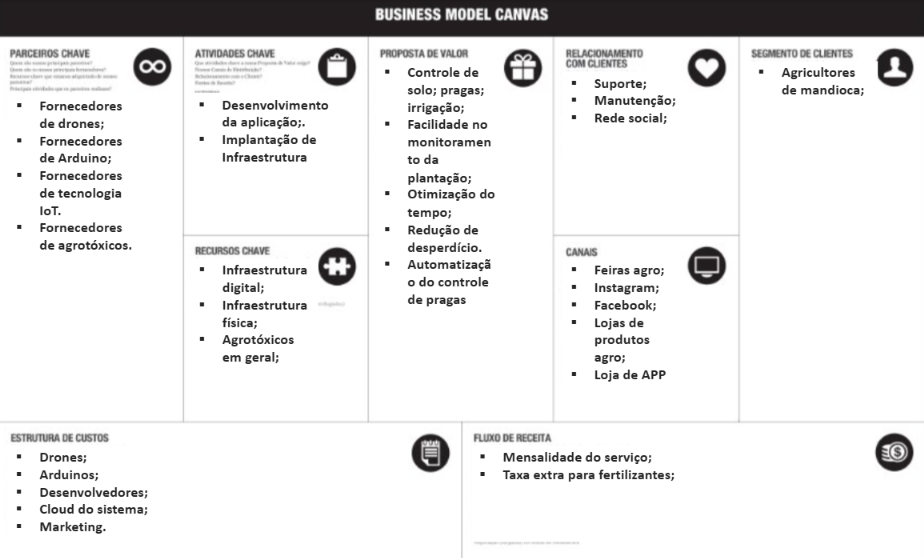
\includegraphics[width=\textwidth]{imgs/canva.png}
    \caption{Business Model Canvas da Solução IoT para Cultivo de Mandioca}
    \label{fig:canvas}
\end{figure}

% ===== SWOT =====
\section{SWOT: Análise Estratégica}

A Análise SWOT \cite{oliveira2023} identifica os fatores internos e externos preponderantes para o sucesso do projeto no contexto do agronegócio familiar.

\begin{table}[H]
\centering
\caption{Análise SWOT do Projeto}
\label{tab:swot}
\begin{tabular}{|p{7.2cm}|p{7.2cm}|}
\hline
\multicolumn{2}{|c|}{\cellcolor{secondarycolor!20}\textbf{FATORES INTERNOS}} \\
\hline
\textbf{FORÇAS (Strengths)} & \textbf{FRAQUEZAS (Weaknesses)} \\
\hline
\begin{minipage}[t]{7cm}
\begin{itemize}[leftmargin=*]
    \item Solução de baixo custo para o produtor
    \item Monitoramento em tempo real (umidade/temperatura)
    \item Foco nas dores do cultivo da mandioca
    \item Interface simplificada e intuitiva
\end{itemize}
\end{minipage}
&
\begin{minipage}[t]{7cm}
\begin{itemize}[leftmargin=*]
    \item Dependência de fornecedores de hardware
    \item Recursos financeiros iniciais limitados
    \item Necessidade de validação em campo
\end{itemize}
\end{minipage}
\\
\hline
\multicolumn{2}{|c|}{\cellcolor{secondarycolor!20}\textbf{FATORES EXTERNOS}} \\
\hline
\textbf{OPORTUNIDADES (Opportunities)} & \textbf{AMEAÇAS (Threats)} \\
\hline
\begin{minipage}[t]{7cm}
\begin{itemize}[leftmargin=*]
    \item Crescimento da agricultura de precisão
    \item Incentivos à agricultura familiar e sustentabilidade
    \item Redução do desperdício de insumos
\end{itemize}
\end{minipage}
&
\begin{minipage}[t]{7cm}
\begin{itemize}[leftmargin=*]
    \item Instabilidade de conectividade no campo
    \item Resistência inicial à adoção tecnológica
    \item Variações climáticas extremas danificando sensores
\end{itemize}
\end{minipage}
\\
\hline
\end{tabular}
\end{table}

\subsection{Recomendações Estratégicas}
\begin{itemize}
    \item \textbf{Forças + Oportunidades:} Utilizar hardware acessível para acelerar a entrada em cooperativas de produtores.
    \item \textbf{Fraquezas + Ameaças:} Planejar caixas de proteção robustas para os sensores e implementar armazenamento em cache local quando a internet oscilar.
\end{itemize}

% ===== UX/UI =====
\section{UX/UI: Design de Interface e Experiência do Usuário}

O design visual foi estruturado sob uma estética moderna em modo escuro com tons terrosos, associando a sobriedade tecnológica às características naturais da cultura da mandioca.

\subsection{Guia de Cores da Aplicação}

\begin{table}[H]
\centering
\caption{Paleta de Cores do Projeto Obelisk}
\label{tab:cores}
\begin{tabular}{|l|c|l|l|}
\hline
\textbf{Classificação} & \textbf{Amostra} & \textbf{Código HEX} & \textbf{Aplicação no Sistema} \\
\hline
Primária & \colorbox{colorPrimaria}{\phantom{AAA}} & \#c7a566 & Botões de ação, destaques e acentos visuais \\
Fundo & \colorbox{colorFundo}{\phantom{AAA}} & \#232323 & Background principal da aplicação / website \\
Títulos e Textos & \colorbox{colorTexto}{\phantom{AAA}} & \#e3e3e3 & Tipografia, títulos de seções e subtítulos \\
Apoio / Secundária & \colorbox{colorSecundaria}{\phantom{AAA}} & \#68532c & Borda de cartões, divisores e botões secundários \\
Clara & \colorbox{colorClara}{\phantom{AAA}} & \#fffcf3 & Contrastes altos e elementos de relevância \\
\hline
\end{tabular}
\end{table}

% ===== WEBSITE =====
\section{Website: Estrutura e Especificações Técnicas}

O portal institucional da \textbf{Obelisk} apresenta a identidade da equipe, a visão estratégica e os projetos tecnológicos voltados à agricultura de precisão e IoT[cite: 1].

\subsection{Interface do Website}

A página inicial do portal adota o conceito \textit{dark mode} para garantir conforto visual e sofisticação, destacando o lema institucional e os projetos desenvolvidos para a cultura da mandioca[cite: 1].

\subsection{Mapa do Site (Arquitetura de Informação)}

A navegação da plataforma divide-se nas seções principais do menu superior, conduzindo o usuário desde a proposta de valor até as formas de contato[cite: 1]:

\begin{figure}[H]
\centering
\begin{tikzpicture}[
    level 1/.style={sibling distance=2.8cm, level distance=1.6cm},
    every node/.style={rectangle, draw=secondarycolor, rounded corners, 
                       fill=secondarycolor!15, 
                       text width=2.4cm, 
                       align=center,
                       font=\small}
]
\node[fill=secondarycolor!30, font=\small\bfseries] {Obelisk\\(Home)}
    child {node {Início}}
    child {node {Sobre}}
    child {node {Consultoria}}
    child {node {Projetos}}
    child {node {Contato}};
\end{tikzpicture}
\caption{Estrutura de navegação do website institucional Obelisk}
\label{fig:sitemap}
\end{figure}

% ===== MODELAGEM E DIAGRAMAS =====
\section{Diagramas UML e Banco de Dados}

Esta seção detalha as regras de negócio, funcionalidades e a persistência dos dados coletados pelos sensores no campo.

\subsection{Diagrama de Casos de Uso}

O diagrama de casos de uso ilustra a interação entre os atores (Administrador, Cliente/Produtor e Sensores) com as funções de monitoramento, emissão de alertas e fertilização.

\begin{figure}[H]
    \centering
    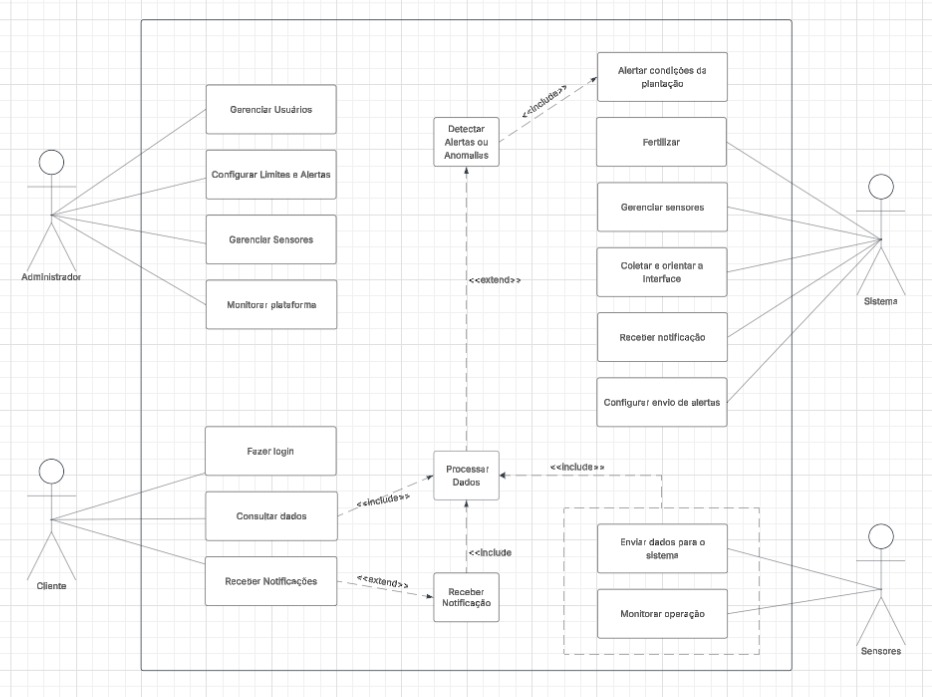
\includegraphics[width=\textwidth]{imgs/diagrama-de-uso.jpeg}
    \caption{Diagrama de Casos de Uso do Sistema IoT}
    \label{fig:use-case}
\end{figure}

\subsection{Modelo Entidade-Relacionamento (Banco de Dados)}

O modelo conceitual do banco de dados representa o vínculo entre clientes, plantações cadastradas, leituras dos sensores, relatórios e geração de alertas.

\begin{figure}[H]
    \centering
    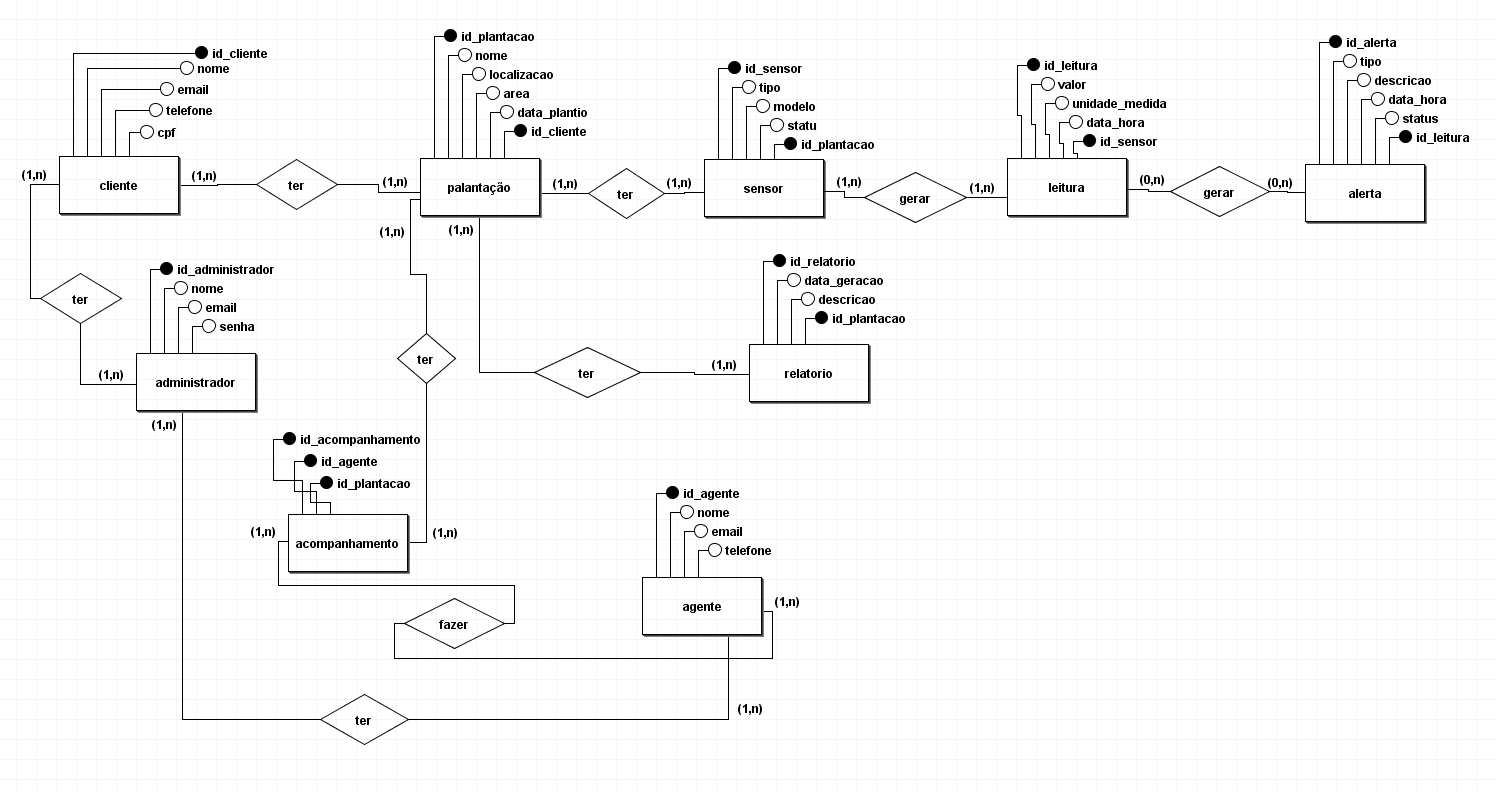
\includegraphics[width=\textwidth]{imgs/banco-dadoos.png}
    \caption{Diagrama Entidade-Relacionamento do Banco de Dados}
    \label{fig:database-er}
\end{figure}

% ===== DEVOPS E INFRAESTRUTURA =====
\section{Infraestrutura, Redes e Conectividade IoT}

\subsection{Topologia de Rede dos Sensores}

A arquitetura de aquisição de dados é composta por microcontroladores, sensores de solo/ambiente e infraestrutura de rede para tráfego das informações até o servidor central.

\begin{figure}[H]
    \centering
    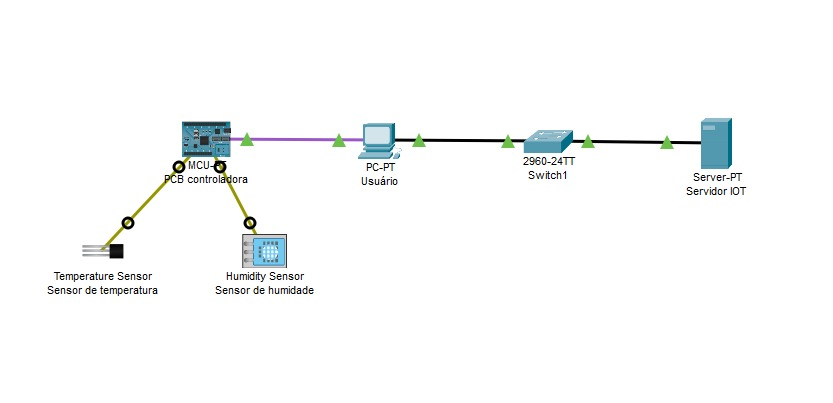
\includegraphics[width=\textwidth]{imgs/diagrama-de-redes.jpeg}
    \caption{Topologia de Rede e Arquitetura de Comunicação IoT}
    \label{fig:rede-iot}
\end{figure}

\subsection{Detalhamento dos Dispositivos da Topologia}

\begin{itemize}
    \item \textbf{Sensores de Campo:} Sensores de temperatura e umidade dedicados à coleta periódica das variáveis do solo e clima da plantação de mandioca.
    \item \textbf{MCU / Placa Controladora:} Microcontrolador responsável por ler os sinais dos sensores analógicos/digitais e transmitir os pacotes de dados.
    \item \textbf{Gateway / Estação do Produtor (PC):} Equipamento que recebe as leituras e realiza o encaminhamento para a infraestrutura de rede local.
    \item \textbf{Switch e Servidor IoT:} Roteamento e armazenamento dos dados para alimentação dos dashboards e regras de alerta.
\end{itemize}

\newpage
\section*{Conclusão}

Os artefatos apresentados neste documento consolidam o planejamento técnico, conceitual e arquitetural do projeto integrador. A solução integra sensores de baixo custo com modelagem relacional e casos de uso voltados a apoiar decisões agrícolas cruciais para a cultura da mandioca.

\vspace{1cm}
\noindent\rule{\textwidth}{0.5pt}

\newpage
\addcontentsline{toc}{section}{Referências}
\bibliographystyle{abntex2-alf}
\bibliography{referencias}

\end{document}